\documentclass[12pt,oneside,final]{fithesis2}
\usepackage[english]{babel}
\usepackage[utf8]{inputenc}
\usepackage[T1]{fontenc}
\usepackage[backend=biber,sorting=none]{biblatex}
\addbibresource{bibliography.bib}
\usepackage[plainpages=false,pdfpagelabels,unicode,hidelinks]{hyperref}
\usepackage[final]{graphicx}
\thesistitle{Mobile Access to jBPM Console}
\thesissubtitle{Bachelor thesis}
\thesisstudent{Tomáš Livora}
\thesiswoman{false}
\thesisfaculty{fi}
\thesisyear{2014}
\thesisadvisor{RNDr. Adam Rambousek}
\thesislang{en}

\begin{document}
\FrontMatter
\ThesisTitlePage

\begin{ThesisDeclaration}
\DeclarationText
\AdvisorName
\end{ThesisDeclaration}

\begin{ThesisThanks}
I would like to thank my supervisor... + Jiří Sviták, Mauricio Salatino
\end{ThesisThanks}

\begin{ThesisAbstract}
The aim of the bachelor work is to provide...
\end{ThesisAbstract}

\begin{ThesisKeyWords}
business process, JBoss, jBPM, jBPM Console, mgwt, mobile application, mobile web
\end{ThesisKeyWords}

\tableofcontents

\MainMatter
\chapter{Introduction}
Nowadays, a rapid growth of the market with smart mobile devices like smartphones or tablets can be noticed.
The parameters of these devices are nearly reaching the performance of classic desktop computers.
Unlike them, the mobile devices also offer comfort of mobility so users have an access to their data and applications whenever or wherever they need it.
However, the burden of this feature is lower comfort while using most of the common applications.
Their graphical user interface (GUI) is often optimized just for standard desktop environments and does not take into account lower screen resolution that is typical for mobile devices.
The other problem is much higher finess of the screen which causes that tiny fonts are usually unreadable without zooming in and also makes it difficult to manipulate with very small control components.

The goal of this thesis is to look through the problematics of developing applications optimized for mobile devices, compare advantages and disadvantages of different approaches and find the optimal solution for the jBPM Console\footnotemark\footnotetext{\url{http://www.jboss.org/jbpm/components/console}}.
The mobile version of this application has been proposed on the website of the JBoss community\footnotemark\footnotetext{\url{https://community.jboss.org/wiki/JbpmProjects}} as a further extension of the jBPM project\footnotemark\footnotetext{\url{http://www.jboss.org/jbpm.html}}.
The thesis deals with analysis, design, implementation and testing of the chosen solution which includes creation of a mobile version of this application with predefined subset of its functions like starting new processes or management of user tasks.
As a part of this thesis the integration test suite was also developed.
The resulting product should become a part of the jBPM Console project.
This work does not aim to make a complex review of the given field and is rather focused on the topics relevant to the implementation part.

The thesis starts with an analysis of different approaches to the mobile applications development.
These are divided into three main categories -- native, web and hybrid -- based on their similar features.
Each category is introduced naming its characteristic features.
Then pros and cons of using the given approach are mentioned and the most suitable use case is outlined.
Next chapter deals with business processes, explains related terms and introduces some commonly used standards.
The motivation for using these processes is given and it is described how they are applied to today's business environment.
Then there is explained how business processes can be automated and how modern enterprise applications based on them are developed.
The following sections introduce business process management (BPM) suite called jBPM.
It is described how its workflow engine works and how can be used by developers of enterprise applications.
Also web-based application jBPM Console for managing business processes which is based on the jBPM engine is introduced.
This chapter describes the application only from the user's point of view.
The underlying services that it is powered by are analysed in the next chapter as a part of the analysis and design of mobile application being developed.
There are also mentioned previous attempts to create mobile version of jBPM Console.
Their results together with other factors are considered while choosing the most suitable way of implementing this project.
An adaptive mobile web application is chosen as the final solution.
Next chapter describes the implementation process.
The technologies used are described and some of the most serious problems that occured during this step are mentioned.
The chapter about testing explains what is the main focus while testing this kind of application.
Both unit testing of GWT components and functional testing by Selenium is performed.
The last chapter is a summary of the work done on this project.
The results are presented and plans for future enhancements are outlined.

The outcome of this thesis is a brief overview of the problematics of developing applications optimized for mobile devices.
This knowledge is applied while implementing a mobile version of jBPM Console.
The output of the practical part is a fully functional mobile web application as well as the related test suite.
The author plans to continue working on this project and improve it by implementing some other functionality that is present in the original jBPM Console application.

\chapter{Mobile applications development}
\label{chap:chapter2}
There are many different approaches to the development of mobile applications.
Each of them with its advantages and disadvantages is suitable for another purpose.
To better understand the differences between these approaches, they can be divided into three categories.

\begin{figure}[ht!]
\centering
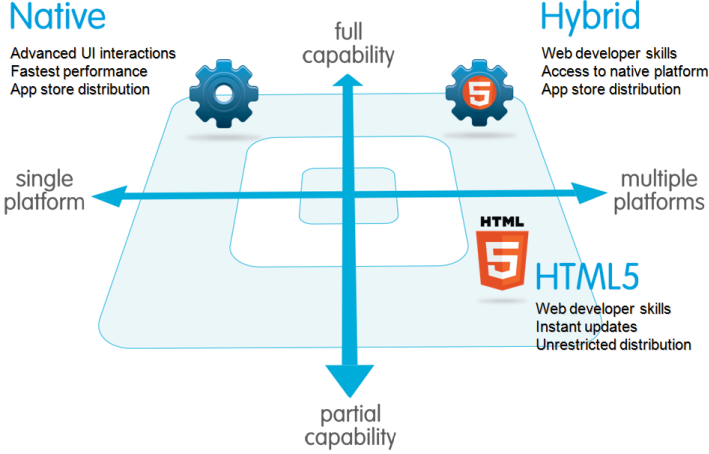
\includegraphics[width=\textwidth]{images/native-html5-hybrid.png}
\caption{Visualization of differences between various approaches to mobile applications development, taken from \cite{developerforce}}
\label{fig:native-html5-hybrid}
\end{figure}

\section{Native applications}
Native applications are designed for the specific platform, e.g. Android, BlackBerry, iOS or Windows Phone.
These applications are installed directly into the target device and are distributed by online markets which are usually platform-specific and offer free as well as paid content.
The examples of such stores are App Store\footnotemark\footnotetext{\url{http://store.apple.com}}, BlackBerry World\footnotemark\footnotetext{\url{http://appworld.blackberry.com}}, Google Play\footnotemark\footnotetext{\url{https://play.google.com/store}} or Windows Phone Store\footnotemark\footnotetext{\url{http://www.windowsphone.com/en-us/store}}.

While developing a native application you have a full access to all the advanced features of the chosen platform like special hardware or operating system-specific functions.
Such software has much better performance than the one created using other approaches because of the lower level of abstraction.
Because these applications are distributed by the mentioned markets, they can be easily monetized.
The presence in the market also allows the discoverability of the work of lesser-known authors (or companies) as users can find all applications on one place.
Another advantage of the centralized application market under the control of the company which develops given platform is that it ensures the quality and safety of the applications.

On the other hand sometimes there may be a conflict between the author's idea of licensing, pricing or updating policy of the application and the rules that must be followed to place the application into the market.
In such cases it is much more difficult to distribute native applications without using the market because the third-part applications are often considered as a security hole and their installation is not allowed by default.
Another problem might be the fact that every platform has its own set of development tools, programming languages and software development kits (SDKs), which make it practically impossible to create cross-platform applications.
This means that a new application needs to be created for each platform which increases the costs of the development proccess.
Users can also use older versions of the application which may bring some additional problems especially when developers add some new functionality to the application that is communicating with the remote devices.
In such cases there is a need for backward compatibility between the different versions.
This may prevent developers from making significant changes and slow down the whole development process.

\section{Mobile web applications}
Mobile web applications are special web pages optimized for mobile devices.
They take into account the limitations and differences of these devices in comparison with desktop computers.
These include smaller screen size, higher fineness of the display, absence of mouse and keyboard, presence of touch control and limited computation power.
But the basic principles of all web pages are also applied in this case.
So you can still find HyperText Markup Language (HTML), Cascading Style Sheets (CSS) and JavaScript on the client's side and the server-side functionality implemented in any suitable language, e.g. PHP, Ruby, Python, Perl or even Java.

The biggest advantage of this approach in comparison with the native applications is that developers do not need to maintain more versions of the application.
This does not only mean that there is one common version for all platforms as users access the application using the web browser.
It also means that all users use the latest version of the application as it is the only one deployed on the server at the time.
This is a significant factor in reducing the development costs as it allows developers not to bother with a backward compatibility so much and make big changes more quickly.
Another important advantage is the fact that developers are not limited by a particular programming language and tools provided for the specific platform.
On the server side they can use any programming language that is supported by the server with any framework or third-part libraries.

However, some new problems might appear when designing mobile web applications.
As users might use various web browsers in different versions there is a need to optimize the application for several versions of all commonly used browsers.
Another thing is the monetizing of this kind of application.
The developers have to set up the advertisements on their own.
They also have to implement their own solution to charge users for using the application.

When designing a mobile web application it is often created as a subset of the funcionality of an existing web application.
In such cases there is usually an intension to somehow connect these two versions to support uniformity and avoid code duplicates.
Nowadays there are basically two ways how to integrate them to one final solution.

\subsection{Responsive web design}
Responsive web design is a technique for developing web applications optimized for different types of devices.
It uses mostly CSS but also JavaScript to adapt the page content to the actual size of the browser's window. \cite{marcotte11}
This technique is suitable when developing a mobile version side-by-side with the full web application.

\subsection{Adaptive delivery}
Adaptive delivery is very similar to the responsive web design.
The main difference is the time when it is decided how the requested page will look like.
While using responsive design it is decided on the client's side by CSS and JavaScript according to the browser's window size, the adaptive delivery is based on different principle.
A type of the client's device is recognized on the server side and only a page for this type of device is sent to the client.
This reduces the amount of incoming traffic on the client side.
It also allows developers to include only relevant parts of the original application in the mobile version.
Some actions might be very difficult to perform on the mobile device so they are likely not to be used and can be ommited from the mobile version.
This approach is prefered to be used also in situations when there is an existing application which is too complex to be changed using the techniques of responsive web design.

\section{Hybrid applications}
Hybrid applications combine the best features of the previous two approaches.
They allow developers to create cross-platform applications that can use some advanced functionality of each platform.
This is achieved by adding another layer which provides JavaScript application programming interface (API) that is common for all platforms.
This API's calls are then translated to native platform-specific API calls.
Such applications are usually written in HTML, CSS and JavaScript.
Then they are packaged as a typical native applications for each platform which means they can be distributed by markets.

The biggest advantage of this approach is that you write only one common code for all platforms.
Developers do not have to learn to use platform-specific tools.
They just get by with the basic web development skills and the knowledge of the provided JavaScript API which allows them to use functions like accelerometer, camera, compass, contacts, file storage, geolocation or notifications.

The drawback of this solution might be the fact that even though you produce applications built for the given platform they do not reach the performance of the native ones.
%\subsection{Web wrapper}
%\subsection{Web-to-native converter}
%\subsection{Native JavaScript API}

\chapter{Business processes and jBPM}
Before designing a mobile version of jBPM Console it is very essential to know what is this application about and how it works.
This chapter explains what business processes are, where they are used and how they can be automated. Also the jBPM engine is introduced and web-based jBPM Console is described both from the users' and developers' point of view.

\section{Business processes}
A business process is a sequence of steps that need to be performed in order to accomplish an organizational goal.
From the technical point of view it can be described as a collection of activities or tasks mutually connected to a logical structure ordered by their time continuity.
Thanks to that a business process can be visualized as a flowchart\footnotemark\footnotetext{A flowchart is a type of diagram used to visualize a process. The individual steps of this process are displayed as various boxes which are connected to each other with arrows determining their order.}.

Nowadays, business processes are so complex and regularly changed that it is practically impossible to hardcode them into the applications and be efficient while adapting to the changes at the same time.
That is why business process management (BPM) tools are used. % BPM vysvetlene uz v uvode
They take control of the maintenance of your business processes and provide API through which your application can easily manipulate with these processes.
This allows developers to focus on the application itself because they do not need to adapt it to the changes in business processes as it is a role of the used BPM tool.

\section{BPMN}
In the past it was usual that every BPM suite implemented and used its own representation of business processes.
As portability became one of the key issues it was necessary to somehow unify these representations and standardize the final outcome so users would be able to reuse their business processes across different BPM tools.

This is why Business Process Model and Notation (BPMN), a standard maintained by the Object Management Group (OMG), was created.
The latest version, BPMN 2.0, is both a business-friendly diagramming notation and an executable process language. \cite{silver11}
The graphical notation of business processes is very similar to activity diagrams from Unified Modelling Language (UML).
A process model is stored as an Extensible Markup Language (XML) file which besides diagram description contains also other information about the process like its data, messages, task assignments etc.

\begin{figure}[ht!]
\centering
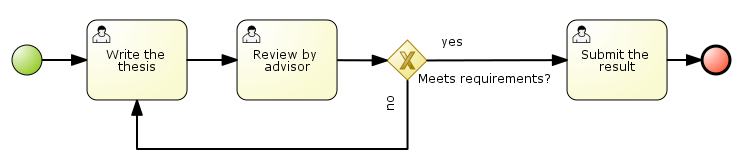
\includegraphics[width=\textwidth]{images/process-example.png}
\caption{Simple example of a business process in BPMN 2.0}
\label{fig:process-example}
\end{figure}

\section{jBPM}
jBPM is an open-source BPM suite developed by the JBoss community.
It can be used to easily model, execute and monitor business processes throughout their life cycle.
The core of jBPM is a light-weight workflow engine that allows users to execute business processes described using the BPMN 2.0 specification.
It can be both embedded in an application or run as a service which users can make use of through the remote APIs.
Besides the core engine, jBPM project also includes other components like a web-based workbench which provides graphical user interface (GUI) for complex management of business processes and Eclipse\footnotemark\footnotetext{\url{https://www.eclipse.org/}} tooling for modeling, testing and debugging of processes.
\cite{jbpm6overview}

\subsection{Core Engine}
The core jBPM engine provides KIE\footnotemark\footnotetext{KIE stands for Knowledge Is Everything.} API \cite{jbpm6api} to control the execution of business processes.
To start working with processes it is first necessary to set up Runtime Environment.
The most important thing here that needs to be specified is a list of process definition files.
These definitions are parsed and stored in a form which allows fast automated execution.
After that Runtime Manager, which is resposible for delivering instances of Runtime Engine, can be created.
Runtime Engine encapsulates the two most important elements of the jBPM engine -- KIE Session and Task Service.
KIE Session provides an interface to communicate with the engine.
It allows users to start new processes, manipulate with the running ones or get some information about those that has already finished.
\cite{jbpm6engine}

\subsection{Task Service}
The Task Service is a special part of the engine responsible for human task management.
A human task (or user task) is an activity type from BPMN 2.0 specification which needs to be executed by human actor.
Human tasks are used to signalize that users are working on something outside of the system or just to get inputs from them.
Every task is assigned to a specific actor or a group of actors who can claim it and start working on it.
The human task itself has its own life cycle which consists of several states.
The simplified version containing only states relevant to the use cases in jBPM Console is visualized in the figure~\ref{fig:task-lifecycle}.
For a more complex description including all possible states and transitions between them see the jBPM Documentation \cite{jbpm6tasklife} or WS-HumanTask Specification \cite{ws-humantask}.

\begin{figure}[ht!]
\centering
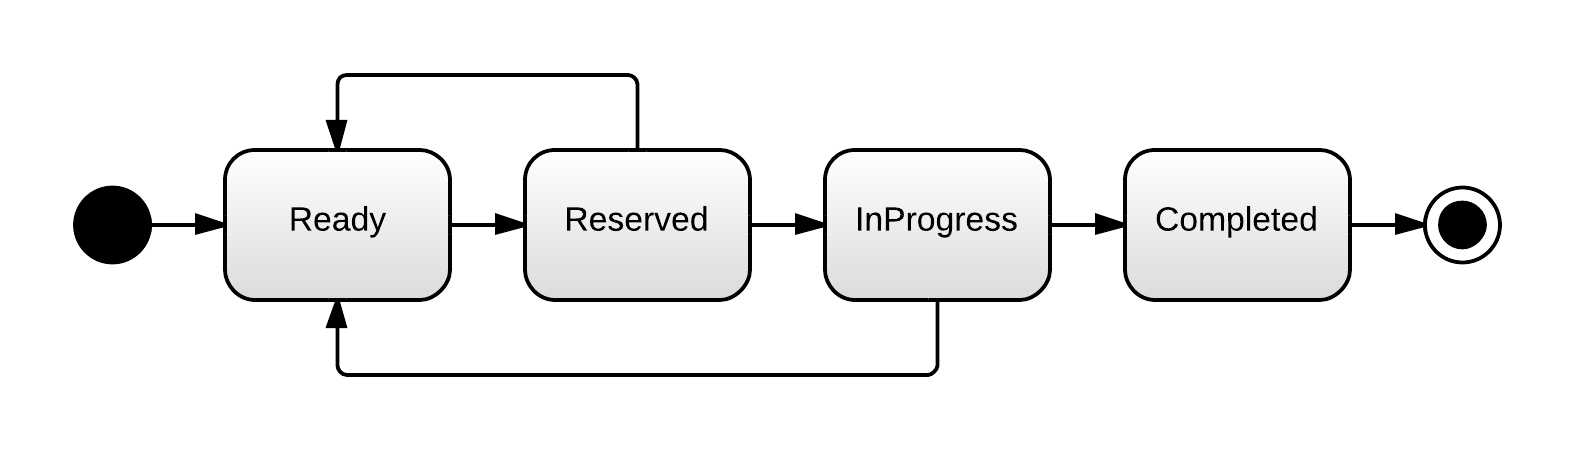
\includegraphics[width=\textwidth]{images/task-lifecycle.png}
\caption{Simplified version of a human task life cycle}
\label{fig:task-lifecycle}
\end{figure}

The Task Service provides a simple API that allows users to handle human tasks.
Using this API tasks can be claimed, started and completed by a user or delegated to someone else.
While completing a task users are able to pass some parameters.
These can be further processed or mapped directly to the process variables.
This is how the interaction between a user and a process instance is ensured and how user actions can influence the following steps in the process execution.

\section{jBPM Console}
The jBPM Console is a web-based tool built on the top of the jBPM services.
It is composed of several components like Guvnor, Designer, Form Modeller and Dashboard.
All this projects grouped together form one unified environment for assets management, business process modeling, managing process runtime and business activity monitoring.

\begin{figure}[ht!]
\centering
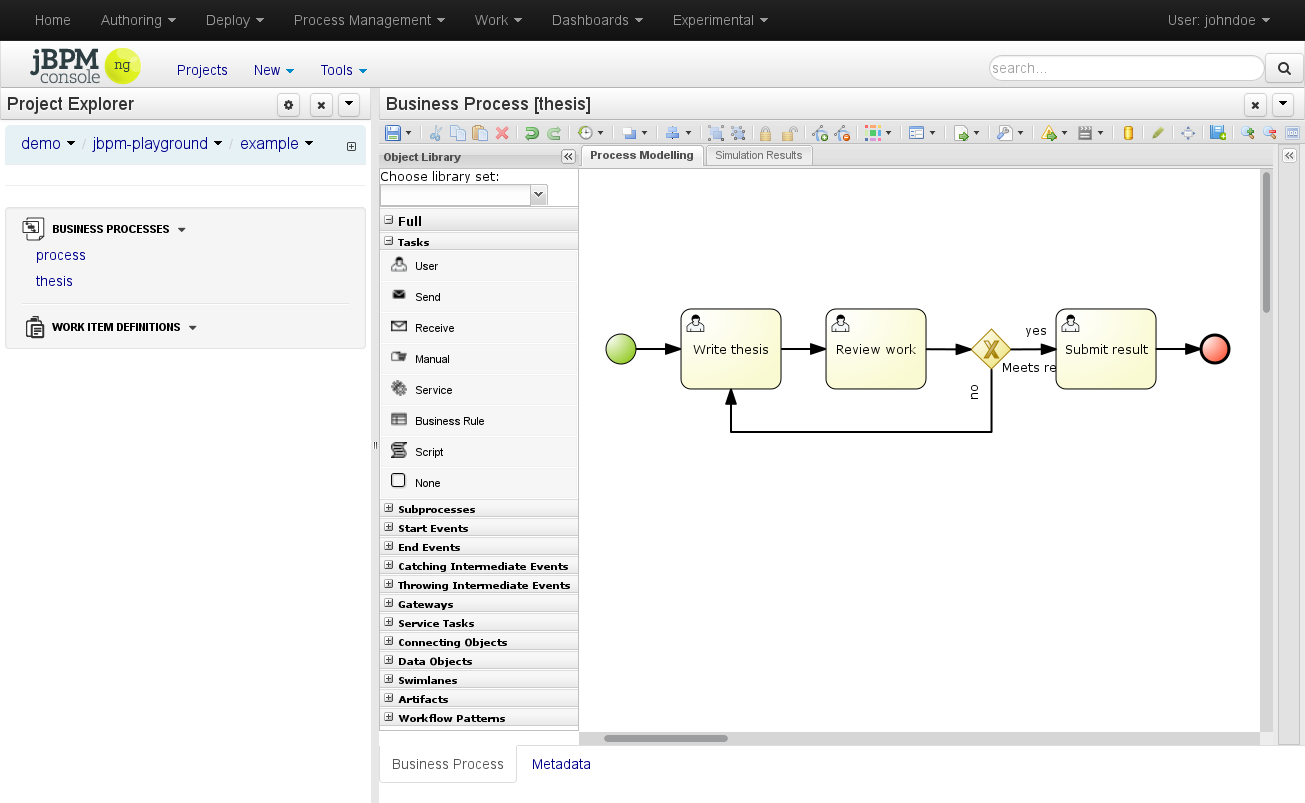
\includegraphics[width=\textwidth]{images/jbpm-console.png}
\caption{Process designer in jBPM Console}
\label{fig:jbpm-console}
\end{figure}

\subsection{Graphical User Interface}
The GUI of the jBPM Console consists of several perspectives.
Each one of them represents one step in the process life cycle.

Authoring perspective is based on the Guvnor component and allows users to manage business assets.
Individual files are stored in a virtual file system (VFS) based on Git\footnotemark\footnotetext{Git is a distributed version control system -- \url{http://git-scm.com/}} repositories.
%These repositories are organized into bigger structures called organizational units.
Users can create a new repositories or clone the remote ones.
Maven\footnotemark\footnotetext{Maven is a software project management tool -- \url{http://maven.apache.org/}} projects are created inside these repositories to simplify organization of the files.
Within these projects several types of new files can be created from which the most important are business process definitions in BPMN 2.0 format and task as well as process forms.
Processes can be edited in their graphical representation by the Designer.
This editor allows users to easily model business processes using the drag\&drop.
After the editing is done a project can be built and deployed so the individual processes within it become ready to be started.

All deployed projects can be seen in a list which is a part of the Deploy perspective.
Users are able to undeploy these projects or create a new deployment unit.

Processes from the deployed projects are all listed in the process definitions list which is a part of the Process Management perspective.
For each process definition there are options to start it as a new process, view its flowchart representation or view all of its instances.
If a process is started a user is prompted to fill in the process form which consists of some input fields.
%if there are any defined.
These inputs can be for example used to initialize process variables.
All process instances are listed in the process instance list where they can be easily controlled.
A running process can be aborted or a signal can be sent to it by a user.
The history of the process variables can also be viewed here.

The Tasks perspective is the one responsible for human tasks management.
Users can view all the tasks that belongs to them or to the groups they are members of.
These tasks are usually created as a result of business process execution but users are also able to create their own personal tasks which do not participate in any process.
Several actions can be executed on these tasks like claiming the ones that nobody is working on, starting work on the claimed tasks and completing tasks.
%Form Modeller

From all the perspectives mentioned above the Process Management and Tasks are the only one that will be included in the mobile version.

\subsection{Modular approach}

From the developer's point of view jBPM Console is a modular application.
Easily said almost every perspective is one independent module.
This approach allows developers to combine modules from different projects and create new applications based on current needs without code duplication.
A typical example is KIE Workbench which is basically jBPM Console merged with Drools Workbench.
The result is a complex application for business and rules management with some additional functionality like remote access to its services.

%\subsection{Remote access}


\chapter{Analysis}
To be able to design the right solution for the mobile version of the jBPM Console it is essential to compare pros and cons of different approaches to mobile applications development (described in chapter~\ref{chap:chapter2}) with the requirements of the application being developed.
Then some previous solutions for implementing a mobile version of this application are mentioned and their weaknesses are discovered.
Finally, a solution is drafted which is considered to be the most appropriate according to the previous findings.

\section{Possible options}
There are basically two options how a mobile version of the jBPM Console can be implemented.
Both solutions assume that there is an instance of the jBPM Console or KIE Workbench running on the server and the main difference between them is the way how mobile devices communicate with it.

\subsection{Native and hybrid applications}
%The biggest advantage of native applications is the fact that they run directly on mobile devices and thus their performance is very high and they are also able to use special hardware components.
%However, a mobile version of jBPM Console does not need to use any hardware-specific functions or perform complicated computations.
%The only thing it needs to do is to react to users' actions by calling the appropriate operations using jBPM services.
%The only thing it needs to do is to use the jBPM services to call the appropriate operations as a reaction to users' actions.
%While native applications run completely on mobile devices they cannot use these services directly but need to access them remotely.
%The solution is to use the REST\footnotemark\footnotetext{Representational state transfer (REST) is an architectural style which uses HTTP commands to execute different actions on resources provided by the server. \cite{fielding20}} API provided by KIE Workbench to communicate with the jBPM engine.
%Using this interface application can work with processes and human tasks even though there is no instance of jBPM engine running locally on the mobile device.

%The most significant drawback of this solution is quite difficult maintenance.
%When a new feature is added to the jBPM Console the REST API needs to be updated together with all platform-specific clients.
%This requires a lot of time and effort to both implement the changes and test all client applications.

%This solution also represents the hybrid applications as the result is practically the same.
%They still run directly on mobile devices and thus have to communicate with the KIE Workbench through the REST interface.
%The only difference is that there is no need to write a new application for each platform so the maintenance is a little bit easier.

Although native and hybrid applications are two slightly different approaches to mobile application development in this context there is almost no difference between them.
What is relevant for designing a mobile version of jBPM Console is the environment in which it will run.
Both types of applications run directly on mobile devices.
The only difference is in the development process.
While native applications need to be developed separately for each platform there is only one common code of a hybrid application which is then compiled for each platform.

While these applications run directly on mobile devices there is a need to communicate with KIE Workbench remotely.
This can be achieved by using the REST\footnotemark\footnotetext{Representational state transfer (REST) is an architectural style which uses HTTP commands to execute different actions on resources provided by the server. \cite{fielding20}} API it provides.
Using this interface a client application can execute all common operations with processes or human tasks.
There is practically no difference between executing them through the web GUI of the jBPM Console or using REST calls as the same backend services are called in both cases.

However, this solution has some serious drawbacks.
Not everything can be executed using the REST API.
If there is a need to perform some more complicated commands this interface will have to be extended.
Also every change to the API urges developers to modify all platform-specific clients.

\subsection{Web application}
The jBPM Console itself is a web application.
That means if a mobile version is also a web application it might be directly a part of the jBPM Console.
The maintenance of such solution will be much easier than managing several platform-specific clients.
There is also no problem with the limited interface as in this case the mobile version will have access to the same resources as the original application.
This solution can be also divided into two slightly different approaches.

Responsive web design is the first one.
This approach would require completely refactor all existing pages and change their layout to follow the rules of responsiveness.
In such a big application as jBPM Console this will be a very complicated process requiring a lot of effort and with uncertain result.
In addition, not all the parts of the original application are suitable for mobile devices.
Actions performed on some of them might be quite unpractical to do on these devices.

On the other side, adaptive delivery is an approach when the detection is performed on the server side.
This allows to create completely different screens for mobile and desktop users.
jBPM Console is implemented using the Model–view–presenter (MVP) pattern so there is an option to add new implementations of view interfaces optimized especially for mobile devices.

\section{Previous attempt}
Android + iPhone apps previously developed
\cite{petovsky13}

\section{Suggested solution}

%\section{Architecture draft}

\chapter{Design and implementation}

\section{Design patterns}

\subsection{MVP}

\section{Technologies}

\subsection{GWT}
Google Web Toolkit (GWT)

\subsection{MGWT}

\subsection{Errai}
%CDI

\subsection{UberFire}

\section{Application architecture}

\section{Actual implementation}


%\section{Architecture}

\chapter{Testing}
\section{Automated functional testing}
\section{Selendroid}

\chapter{Summary}

\printbibliography

\end{document}